\begin{figure}[htbp]
\centering
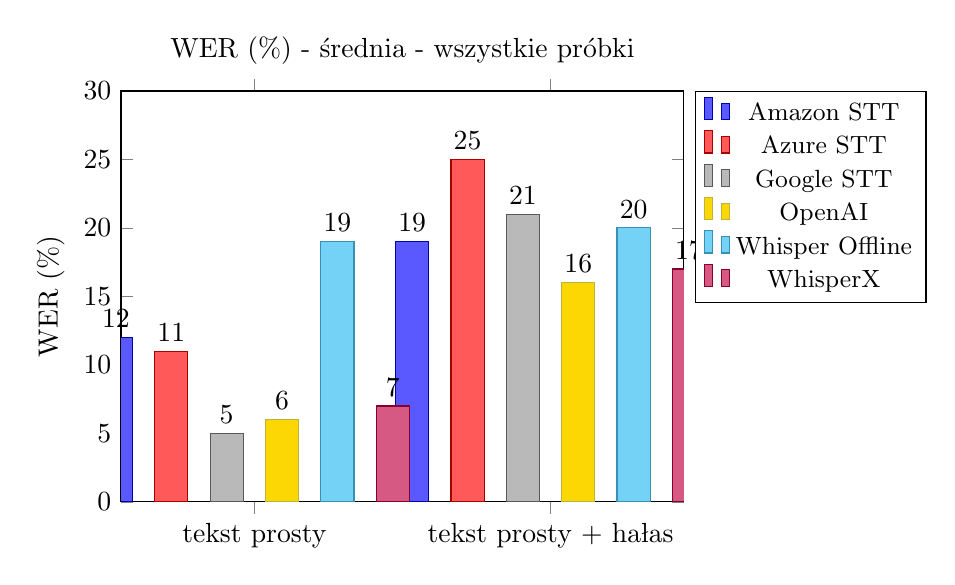
\begin{tikzpicture}
\begin{axis}[
    ybar,
    symbolic x coords={tekst prosty,tekst prosty + hałas},
    xtick=data,
    nodes near coords,
    nodes near coords align={vertical},
    nodes near coords style={
        /pgf/number format/fixed,
        /pgf/number format/precision=0,
    },
    ylabel={WER (\%)},
    ymin=0, ymax=30,
    ytick={0,5,10,15,20,25,30},
    yticklabel={\pgfmathprintnumber[fixed,precision=0]{\tick}},
    ybar=8pt,
    bar width=12pt,
    enlarge x limits=0.45,
    title={WER (\%) - średnia - wszystkie próbki},
    legend style={
        at={(1.02,1)},
        anchor=north west,
        font=\small,
    },
    x tick label style={align=center},
    width=0.72\textwidth,
    height=6.8cm,
]
\addplot[fill=blue!65, draw=blue!65!black] coordinates {
    (tekst prosty,12)
    (tekst prosty + hałas,19)
};
\addplot[fill=red!65, draw=red!65!black] coordinates {
    (tekst prosty,11)
    (tekst prosty + hałas,25)
};
\addplot[fill=gray!55, draw=gray!70!black] coordinates {
    (tekst prosty,5)
    (tekst prosty + hałas,21)
};
\addplot[fill=yellow!75!orange, draw=yellow!70!black] coordinates {
    (tekst prosty,6)
    (tekst prosty + hałas,16)
};
\addplot[fill=cyan!55, draw=cyan!70!black] coordinates {
    (tekst prosty,19)
    (tekst prosty + hałas,20)
};
\addplot[fill=purple!65, draw=purple!70!black] coordinates {
    (tekst prosty,7)
    (tekst prosty + hałas,17)
};
\legend{Amazon STT,Azure STT,Google STT,OpenAI,Whisper Offline,WhisperX}
\end{axis}
\end{tikzpicture}
\caption{Porównanie błędu WER dla badanych modeli ASR w warunkach hałasu.}
\label{fig:wer_cer_comparison_noise}
\end{figure}
